\documentclass[uplatex, a4paper, 12pt, openany, oneside]{jsbook}

\usepackage[dvipdfmx]{graphicx}
\usepackage[dvipdfmx]{color}
\usepackage[dvipdfmx, bookmarks=true, setpagesize=false]{hyperref}
\usepackage{pxjahyper}

\usepackage{thesis}
\usepackage{here}
\usepackage{url}


\thesis{卒 業 論 文}
\title{
  \centering
    \scalebox{1.0}{視覚と行動のend-to-end学習により}
    \vspace{-0.3zh}
    \scalebox{1.0}{経路追従行動をオンラインで模倣する手法の提案}
    \vspace{-0.3zh}
    \scalebox{1.0}{(目標方向による経路選択機能の追加と検証)}
    % \vspace{-0.1zh}
    \vspace{0.5cm}
    \scalebox{0.6}{A proposal for an online imitation method of path-tracking}\\
    \vspace{-0.6zh}
    \scalebox{0.6}{behavior by end-to-end learning of vision and action}\\
    \vspace{-0.6zh}
    \scalebox{0.6}{(Addition of path selection function and verification by target direction)}\\
    \vspace{-0.6zh}
}
\setlength{\textwidth}{\fullwidth}
\setlength{\evensidemargin}{\oddsidemargin}

\date{\today}
\vspace{-15.0zh}
\teacher{林原 靖男 教授}
\vspace{-15.0zh}
\organization{千葉工業大学 先進工学部 未来ロボティクス学科}
\author{19C1101 藤原 柾}
\vspace{-15zh}

\renewcommand{\baselinestretch}{1.2}
\begin{document}

%% Front Matter
\frontmatter{}
%
\chapter{実験}
\label{chap:experiments}
この章では, 1節で我々が行ってきた研究\cite{mech}の実験(以下, 「従来の実験」と称する)を実環境に移行する際に, 新たに顕在化した課題点について述べる. また, 課題を解決するための2つのアプローチを提案し, 実験と検証を行う. 2節では, 実験に簡易的なシミュレータを用いる問題点を述べ, 解決策を提示する. 3節では, 実環境で実験を行い, 実環境における提案手法の有効性を検証する.  
%
%\input{experiments/preface}
%
%!TEX root = ../thesis.tex

\section{実験要件}
実験には下記のコンピュータとソフトウェアを用いた. 

\begin{enumerate}
  \item コンピュータ\\
  OS: Ubuntu 20.04 LTS\\
  ROS: Noetic\\
  CPU: intel Core i7-10700F(4.8GHz/8コア/16スレッド)\\
  DRAM: 32GB DDR4(3200/8GB×4)
  \item nav\_cloning(学習器, 統合環境)\\
  \url{https://github.com/open-rdc/nav_cloning}
  \item waypoint\_nav(移動目標地点, 目標方向を出力)\\
  \url{https://github.com/open-rdc/waypoint_nav}
  \newpage
  \item turtlebot3 関連\\
  \url{https://github.com/open-rdc/turtlebot3}
  \item navigation(ナビゲーションパッケージ)\\
  \url{https://github.com/ros-planning/navigation}
\end{enumerate}

\subsection{実験装置(シミュレータ)}

\begin{itemize}
  \item ロボット

ロボットモデルは前報\cite{okada1}\cite{okada2}と同様, \figref{Fig:waffle_pi}に示すように, TurtleBot3 Waffle\_piへ3つのカメラを追加したモデルを用いる.

\begin{figure}[hbtp]
  \centering
 \includegraphics[keepaspectratio, scale=0.22]
      {images/Waffle_pi.png}
 \caption{TurtleBot3 waffle\_pi with 3 cameras}
 \label{Fig:waffle_pi}
\end{figure}

\item 環境\\
シミュレータ環境として, オープンソースの3DロボットシミュレータGazeboを用いる. \figref{Fig:sim}に示すようなGazebo上で千葉工業大学2号館3階を模した実験環境を対象に実験を行う.

\begin{figure}[hbtp]
  \centering
 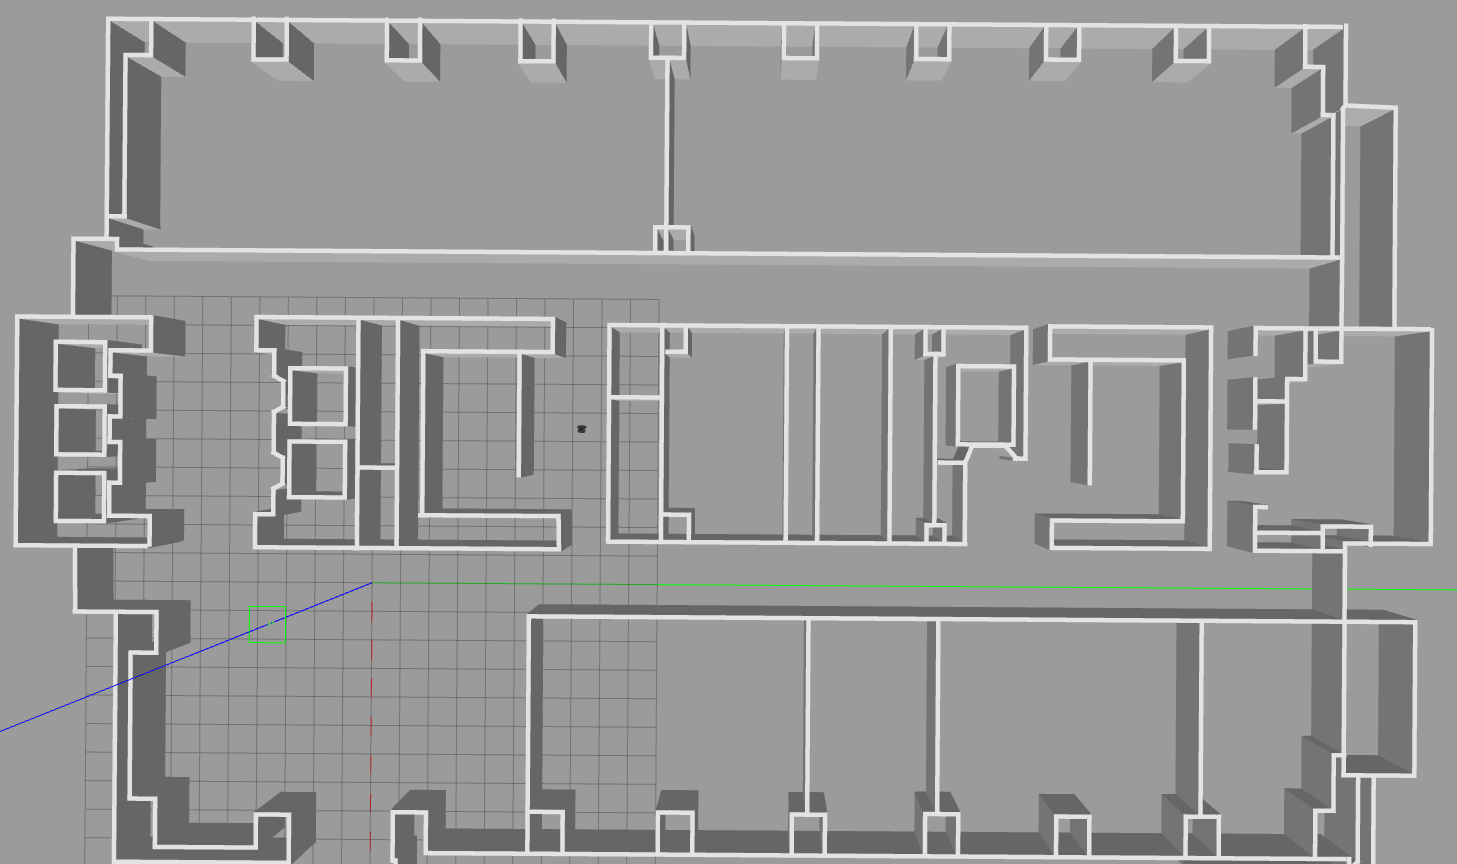
\includegraphics[keepaspectratio, scale=0.12]
      {images/tsudanuma2-3_simorg.png}
 \caption{Experimental enviroment of simulator}
 \label{Fig:sim}
\end{figure}

\end{itemize}

\subsection{実験方法}
\figref{Fig:sim_explain}のA, B地点において, \figref{Fig:select}に示すように侵入する方向が3つあり, 進むことのできる方向が2つあることから, 1箇所につき走行パターンが6つ存在する. 
また, A, B地点では, 目標方向に従って任意の経路を選択することが求められる場所である.
したがって, 実験ではA, B地点で合計12パターンの走行において, 与えた目標方向に従った行動が行えるのかを確認する.

\begin{figure}[hbtp]
  \centering
 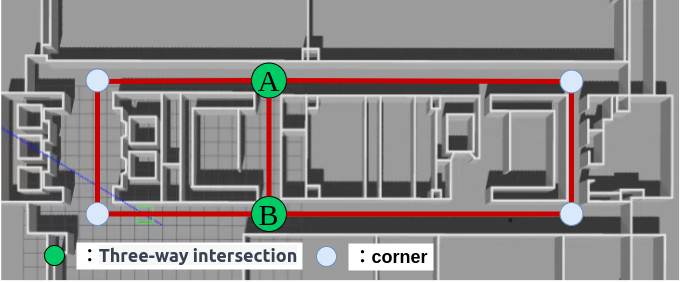
\includegraphics[keepaspectratio, scale=0.5]
      {images/sim_explain.png}
 \caption{Characteristics of passages in the experimental environment on the simulator}
 \label{Fig:sim_explain}
\end{figure}

\begin{figure}[hbtp]
  \centering
 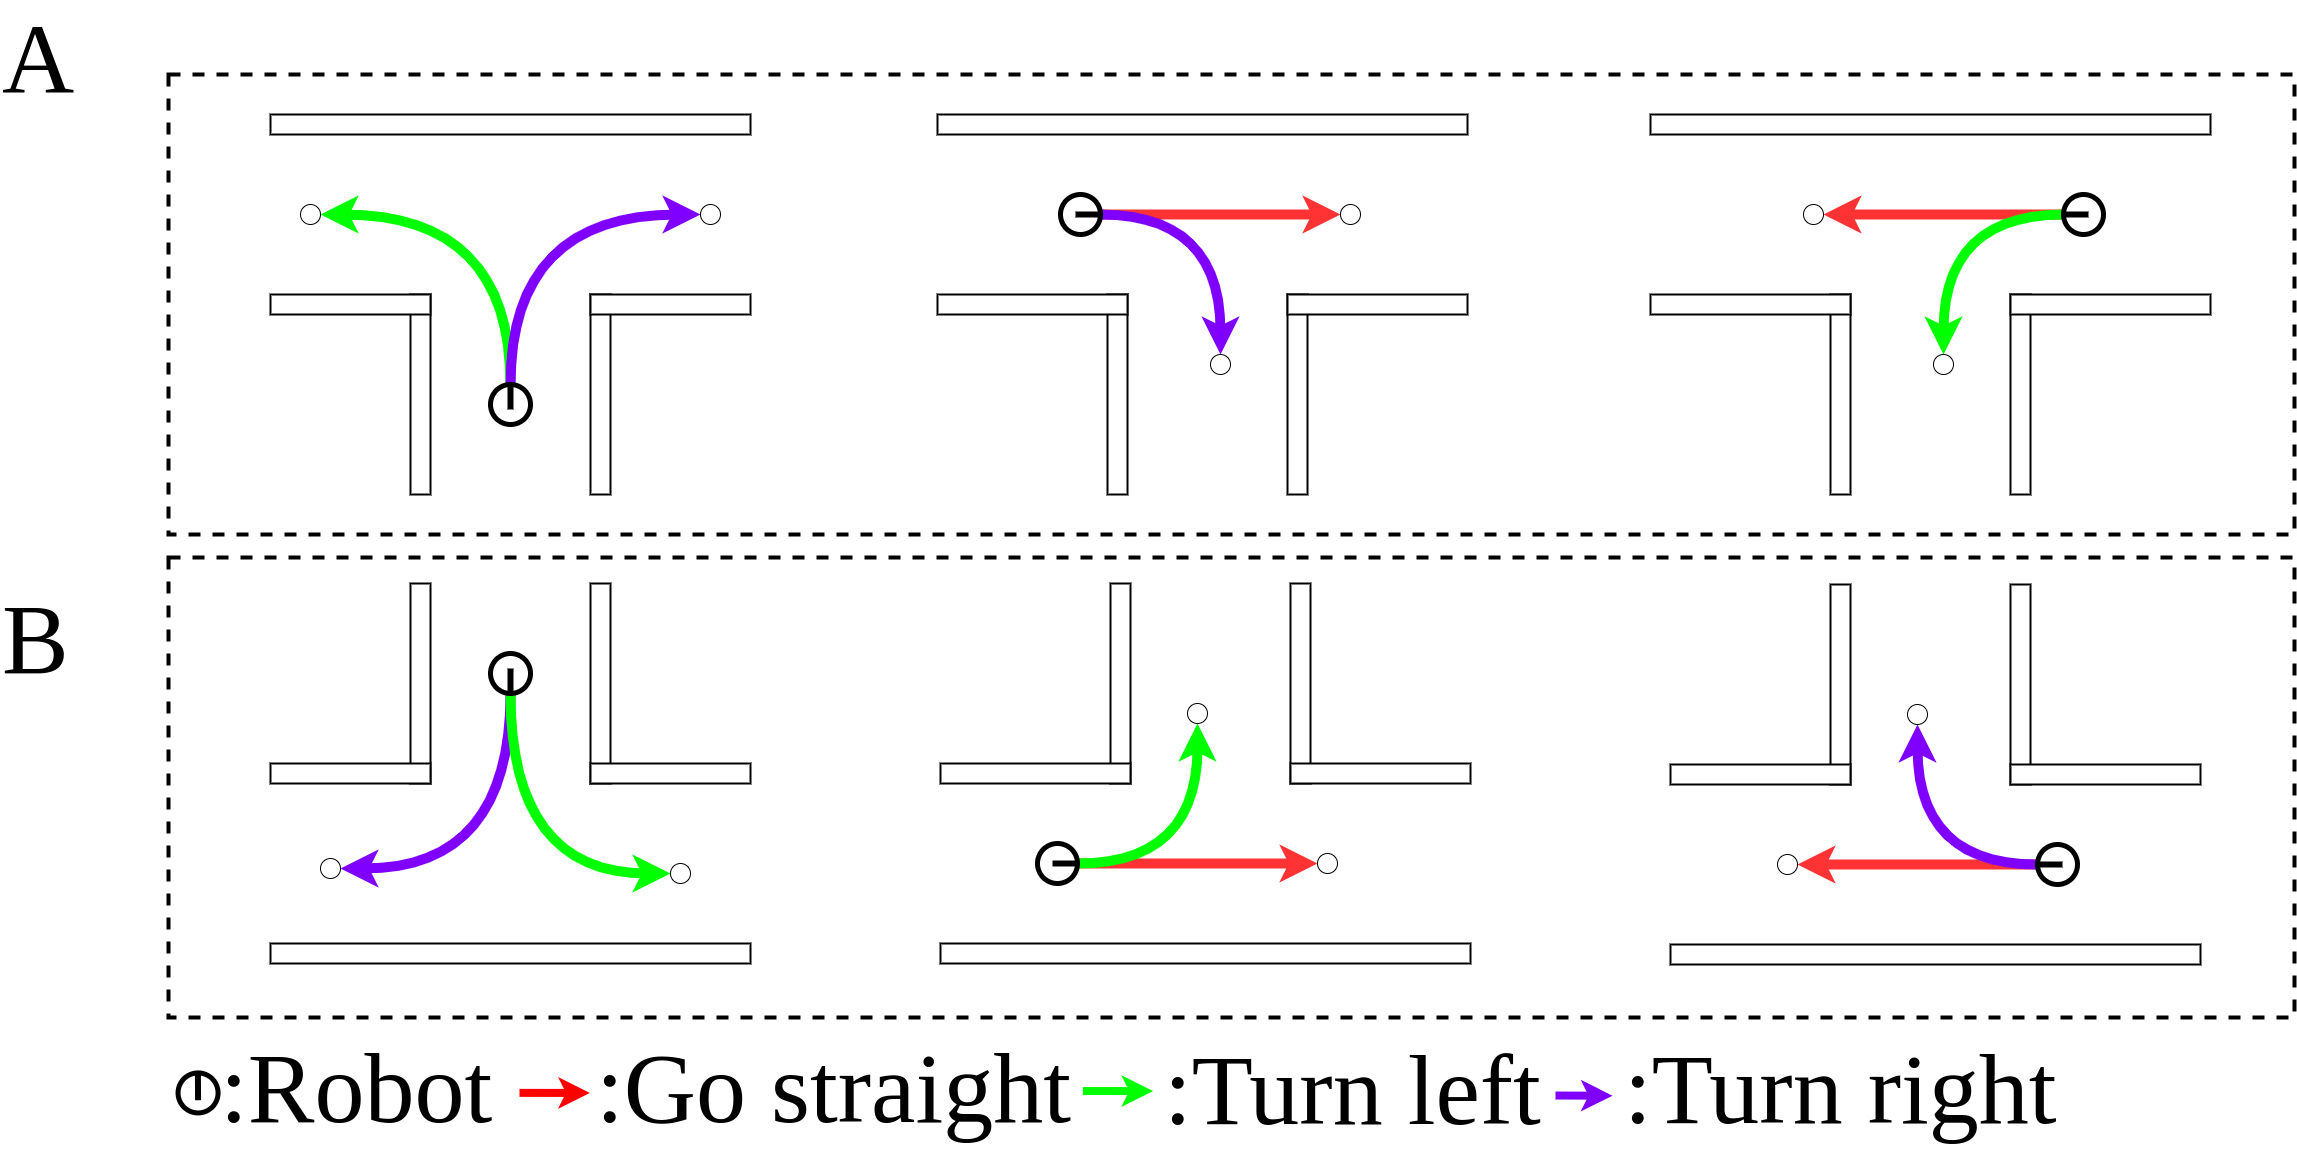
\includegraphics[keepaspectratio, scale=0.15]
      {images/select.png}
 \caption{Moving pattern at points A and B}
 \label{Fig:select}
\end{figure}

全ての走行パターンを網羅するように模倣学習を行うため, \figref{Fig:route}に示すようにaからfまでの経路を繰り返し走行させる. なお, 目標方向はwaypoint\_navから生成され, データセットに加えられる. 学習終了後, テストフェーズに移行するが, 学習時と同様にaからfまでの順番で経路をロボットに走行させる. また, テストフェーズ時にロボットが壁に衝突した場合, 経路の中央にロボットを移動させた後, 走行を再開させる.

\vspace{1cm}

\begin{figure}[hbtp]
  \centering
 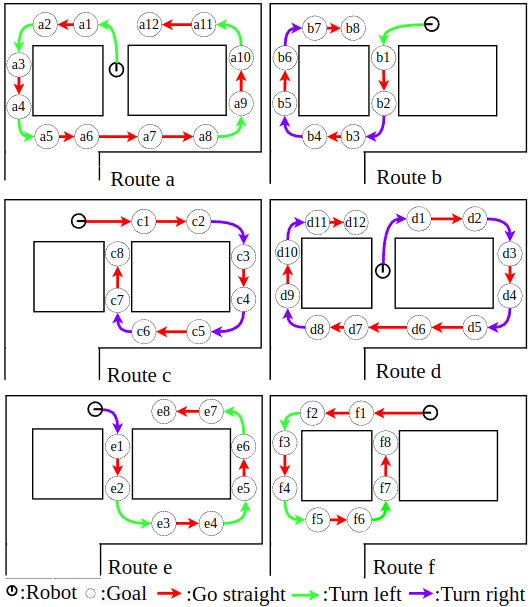
\includegraphics[keepaspectratio, scale=0.6]
      {images/route.png}
 \caption{Moving pattern at points A and B}
 \label{Fig:route}
\end{figure}

\newpage

%!TEX root = ../thesis.tex

\section{課題点と2つのアプローチによる実験}
我々が行ってきた研究では, 簡易的なシミュレータ上で提案手法が有効だと確認されている. そのため, 次の段階として実環境における提案手法の有効性を検証することを試みた. そこで, 新たに顕在化した課題点は以下の2つの点である.

\begin{itemize}
  \item 実験条件(主にカメラ画像に影響を及ぼす光である)を揃える関係上, 実験を行う時間帯を光の変化が少ない夜間に固定する必要があるため, 1日に実験を行える時間が少なく, 1回の学習に何日も費やす必要がある
  \item 長時間の学習に耐えられるだけのバッテリ容量がロボットにない
\end{itemize}

これらの課題点から, 学習時間の短縮が必要であると判断した. そのため, 2つのアプローチを提案し, 学習量を削減する.
\par
この節では, まず, 従来の実験を簡単に紹介する. 次に, 2つのアプローチについての詳細と行った実験を述べる. 最後に, アプローチを試みる前と各アプローチによる実験結果を比較し, 議論を行う.

\subsection{従来の実験}

\begin{itemize}
  \item 実験目的\\
  簡易的なシミュレータ上で, 提案手法の有効性の検証を行う
  \item 実験装置\\
  4.1.1で述べた簡易的なシミュレータ環境とロボットで実験を行った
  \item 実験方法\\
  4.1.2で示した経路を繰り返し走行させる. 学習を60000step実行後, テストフェーズに移行する. テストフェーズで正しい順序で経路を選択し, 走行を行えるか確認する. この一連の流れを10回繰り返し行う.

  \newpage

  \item 実験結果\\
  実験結果を\figref{Fig:60000step}に示す. この図は, それぞれの走行パターンにおいて正しく経路を選択し, 走行できた回数を表している. \tabref{table:result}に全パターンの成功回数を合計した結果を示す. なお, 分母が120であるのはテストフェーズにおいて, 全12パターンからなる経路を走行させ, 評価を行うことを10回繰り返したためである. 
  \par
  \tabref{table:result}に示すように, 目標方向に従って113/120回, 正しい経路を選択する様子が見られた. 

\vspace{1cm}

\begin{figure}[hbtp]
  \centering
 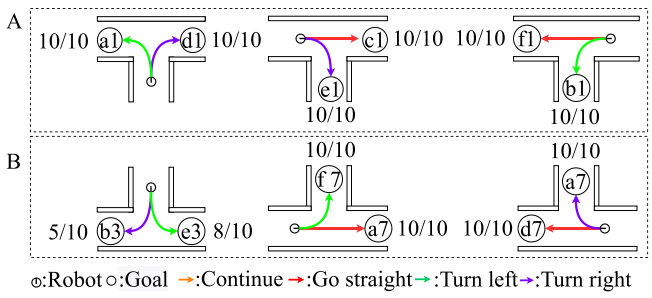
\includegraphics[keepaspectratio, scale=0.5]
      {images/60000step.png}
 \caption{Experimental results for each moving pattern from \cite{mech}}
 \label{Fig:60000step}
\end{figure}

\vspace{1cm}

\begin{table}[hbtp]
  \caption{Experimental results}
  \label{table:result}
  \centering
  \begin{tabular}{|c|c|c|}
    \hline
    Experiments & Step & Total result\\
    \hline
    Conventional & 60000 & 113/120(94.2\%)\\
    \hline
  \end{tabular}
\end{table}

\end{itemize}

\newpage

この従来の実験を基に, 単に60000stepから10000stepに学習量を削減し, 実験した結果を下記に示す.

実験結果を \figref{Fig:10000step} に示す. この図は, それぞれの走行パターンにおいて正しく経路を選択し, 走行できた回数を表している. \tabref{table:result_without} に実験ごとに全パターンの成功回数を合計した結果を示す. \tabref{table:result_without} に示すように, 目標方向に従って 87/120 回, 正しい経路を選択する様子が見られた.

60000stepの実験と成功率を比較すると約22\%ほどの差がある. これでは, 学習量を削減できたとは言い難い. そのため, 後述する2つのアプローチを試みることで成功率の改善を図る.

\vspace{0.5cm}

\begin{figure}[hbtp]
  \centering
 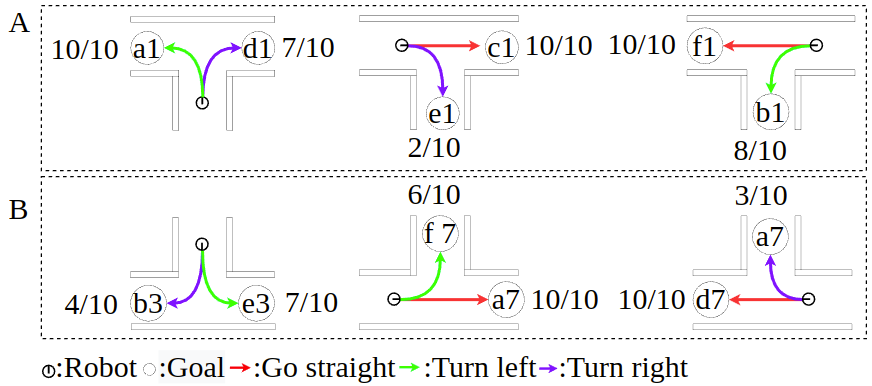
\includegraphics[keepaspectratio, scale=0.43]
      {images/10000step.png}
 \caption{Experimental results for each moving pattern at 10000step by conventional}
 \label{Fig:10000step}
\end{figure}  

\vspace{0.5cm}

\begin{table}[hbtp]
  \caption{Experimental results at 10000step by conventional}
  \label{table:result_without}
  \centering
  \begin{tabular}{|c|c|c|}
    \hline
    Experiments & Step & Total results\\
    \hline
    Conventional & 60000 & 113/120(94.2\%)\\
    \hline
    Conventional & 10000 & 87/120(72.5\%)\\
    \hline
  \end{tabular}
\end{table}

\newpage



\subsection{アプローチ1:データセットに加えるデータの割合変更}
従来の実験における10000stepごとのコマンドに対応するデータ数を\figref{Fig:hist}に示す. \figref{Fig:hist} (a)より, 直進コマンド時のデータ数が圧倒的に多いことがわかる. このデータ数の偏りを解消するため, \figref{Fig:hist} (b)に示すように, 左折と右折コマンドのデータ数を7倍にする. 7倍にするのは, 左折と右折コマンドのデータ数を直進コマンドと同程度にするためである. なお, データ数を何倍にするのが望ましいのか本論文では議論しない. 実験により, データセットに加えるデータ数の割合変更が有効か検証する.

% \begin{figure}[h]
%   \begin{minipage}[b]{0.5\linewidth}
%     \centering
%  \includegraphics[keepaspectratio, scale=0.3]
%       {images/hist_change_org.png}
%  \subcaption{hoge}
%  \label{Fig:hist_org}
% %  \label{Fig:hist_change_org}
% \end{minipage}

%   \begin{minipage}[b]{0.5\linewidth}
%     \centering
%  \includegraphics[keepaspectratio, scale=0.3]
%       {images/hist_change_times7.png}
%  \subcaption{jkofs}
%  \label{Fig:hist_times7}
% %  \label{Fig:hist_change_times7}
%   \end{minipage}
%   \caption{Number of data per command per 10000steps in conventional experiments}
%    \label{Fig:hist}
% \end{figure}

\begin{figure}[h]
  \centering
  \begin{minipage}[b]{67mm}
    \centering
    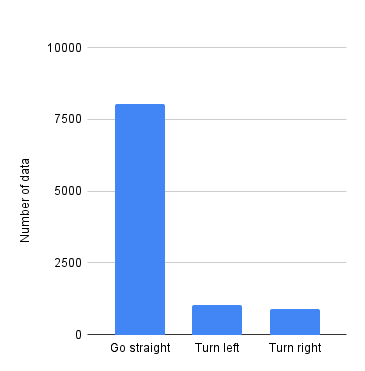
\includegraphics[width=67mm]{images/hist_change_org.png}
    \caption*{(a)}
  \end{minipage} 
  % \newpage
  % \hspace{0.03\columnwidth}
  \begin{minipage}[b]{67mm}
    \centering
    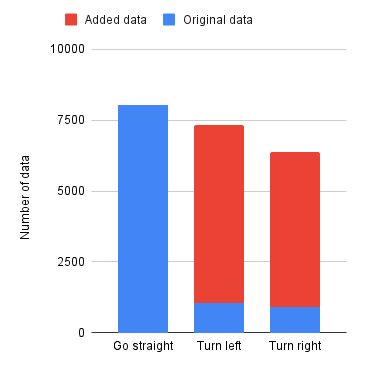
\includegraphics[width=67mm]{images/hist_change_times7.png}
    \caption*{(b)}
  \end{minipage}
  \caption{Number of data per command per 10000steps in conventional experiments}
  \label{Fig:hist}
\end{figure}

\begin{itemize}
  % \item 実験目的\\
  % データセットに加えるデータの割合変更が有効か検証を行う
  \item 実験装置\\
  4.1.1で述べた簡易的なシミュレータ環境とロボットで実験を行った
  \item 実験方法\\
  4.1.2で示した経路を繰り返し走行させる. 学習を10000step実行後, テストフェーズに
  移行する. テストフェーズで正しい順序で経路を選択し, 走行を行えるか確認する. こ
  の一連の流れを10回繰り返し行う.
  \newpage
  \item 実験結果\\
  実験結果を\figref{Fig:10000step_act1.0}に示す. この図は, それぞれの走行パターンにおいて正しく経路を選択し, 走行できた回数を表している. \tabref{table:result3}に実験ごとに全パターンの成功回数を合計した結果を示す. 
  \tabref{table:result3}に示すように, 目標方向に従って99/120回, 正しい経路を選択する様子が見られた. 
  \par
  60000stepの実験と成功率を比較すると約12\%ほど差があり, アプローチ1を試みた結果では成功率が十分だとは言い難い. 次に成功率を改善するため, 後述するアプローチ2を試みた.

  \vspace{0.5cm}

  \begin{figure}[hbtp]
    \centering
   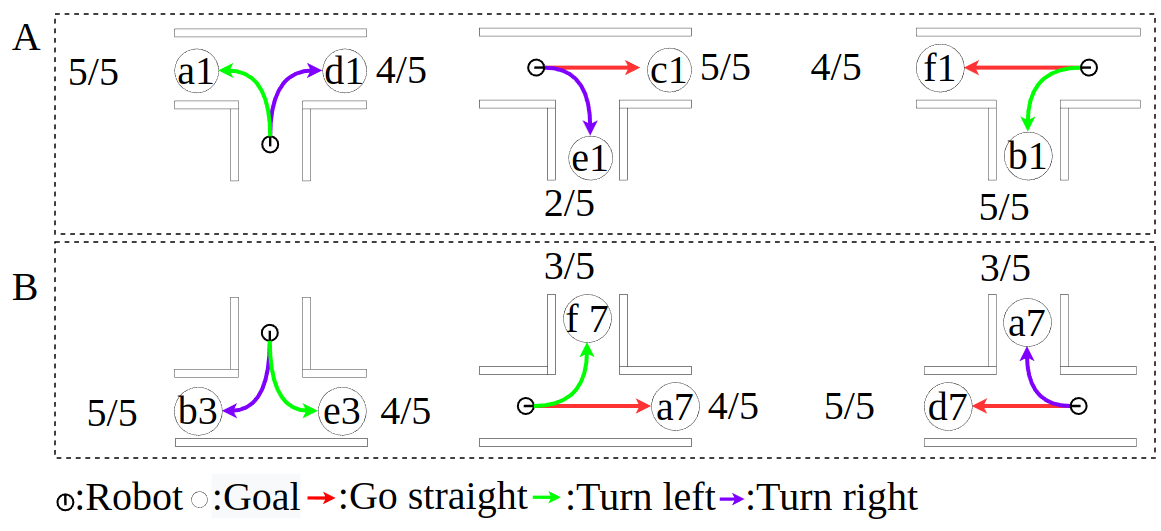
\includegraphics[keepaspectratio, scale=0.5]
        {images/10000step_act1.0.png}
   \caption{Experimental results for each moving pattern by Approach1}
   \label{Fig:10000step_act1.0}
  \end{figure}  
  
  \vspace{0.5cm}

  \begin{table}[hbtp]
    \caption{Experimental results by Approach 1}
    \label{table:result3}
    \centering
    \begin{tabular}{|c|c|c|}
      \hline
      Experiments & Step & Total results\\
      \hline
      Conventional & 60000 & 113/120(94.2\%)\\
      \hline
      Conventional & 10000 & 87/120(72.5\%)\\
      \hline
      Approach1 & 10000 & 99/120(82.5\%)\\
      \hline
    \end{tabular}
  \end{table}

\end{itemize}

\newpage

\subsection{アプローチ2:学習フェーズにおける積極的な蛇行}
清岡ら\cite{kiyooka}により, 目標経路上に加えて離れた状態を学習することが, テストフェーズでの走行に大きな影響を与えるため, 重要だとされている. そのため, より積極的に蛇行を行い, 目標経路から離れた状態を増加させることを検討する. \par
実験で用いているシステムの学習フェーズでは,  \figref{Fig:act1.0}に示すようにロボットが目標経路上付近を走行している場合, 訓練中の学習器へ画像を入力し, 出力される角速度を用いて走行している. この場合に, 目標経路から一定の距離離れると地図を用いたルールベース制御器の走行に切り替わり, 強制的にロボットを目標経路上に戻すように制御を行う. 

\begin{figure}[hbtp]
  \centering
 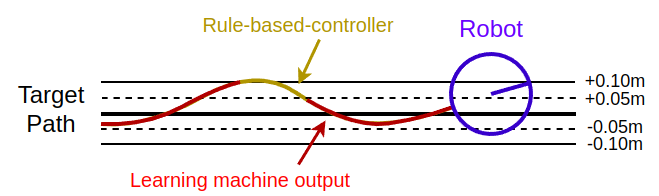
\includegraphics[keepaspectratio, scale=0.58]
      {images/act1.0.png}
 \caption{Moving on the target path}
 \label{Fig:act1.0}
\end{figure}

訓練中の学習器へ画像を入力し, \figref{Fig:3action}のように出力される角速度を1.5倍にする. その結果, \figref{Fig:act1.5}に示すように蛇行する頻度が高くなり, 目標経路から離れた状態をより多く学習できる可能性がある. なお, 得られた角速度を何倍にするのが望ましいのか本論文では議論しない. 実験により, 学習フェーズにおける積極的な蛇行が有効か検証する.

\begin{figure}[hbtp]
  \centering
 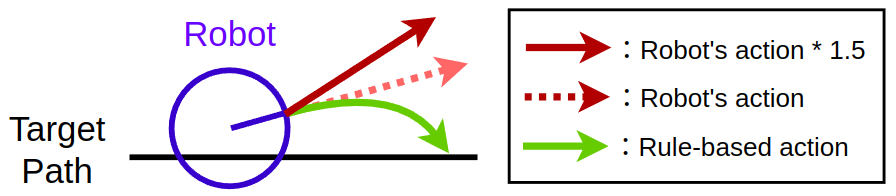
\includegraphics[keepaspectratio, scale=0.43]
      {images/3action.png}
 \caption{Robot behavior}
 \label{Fig:3action}
\end{figure}

\begin{figure}[hbtp]
  \centering
 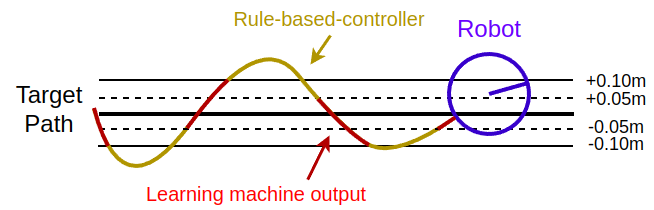
\includegraphics[keepaspectratio, scale=0.58]
      {images/act1.5.png}
 \caption{Moving on the target path attempting approach 2}
 \label{Fig:act1.5}
\end{figure}

\begin{itemize}
  % \item 実験目的\\
  % データセットに加えるデータの割合変更が有効か検証を行う
  \item 実験装置\\
  4.1.1で述べた簡易的なシミュレータ環境とロボットで実験を行った
  \item 実験方法\\
  4.1.2で示した経路を繰り返し走行させる. 学習を10000step実行後, テストフェーズに
  移行する. テストフェーズで正しい順序で経路を選択し, 走行を行えるか確認する. こ
  の一連の流れを10回繰り返し行う.
  \item 実験結果\\
  実験結果を\figref{Fig:10000step_act1.5}に示す. この図は, それぞれの走行パターンにおいて正しく経路を選択し, 走行できた回数を表している. \tabref{table:result4}に実験ごとに全パターンの成功回数を合計した結果を示す. 
  \tabref{table:result4}に示すように, 目標方向に従って109/120回, 正しい経路を選択する様子が見られた. 
  % また, 
  % \par
  % \tabref{table:result4}からアプローチ1の実験より, 成功率が改善していることがわかる. また, 60000stepの実験と成功率を比較した場合, 約4\%ほどの差がある. これには, 以下2つの要因が挙げられる.
  % \begin{itemize}
  %   \item 
  % \end{itemize}
  % そのため, 10000stepから20000stepに学習量を増加し, 実験した結果を下記に示す.

  
  \begin{figure}[hbtp]
    \centering
   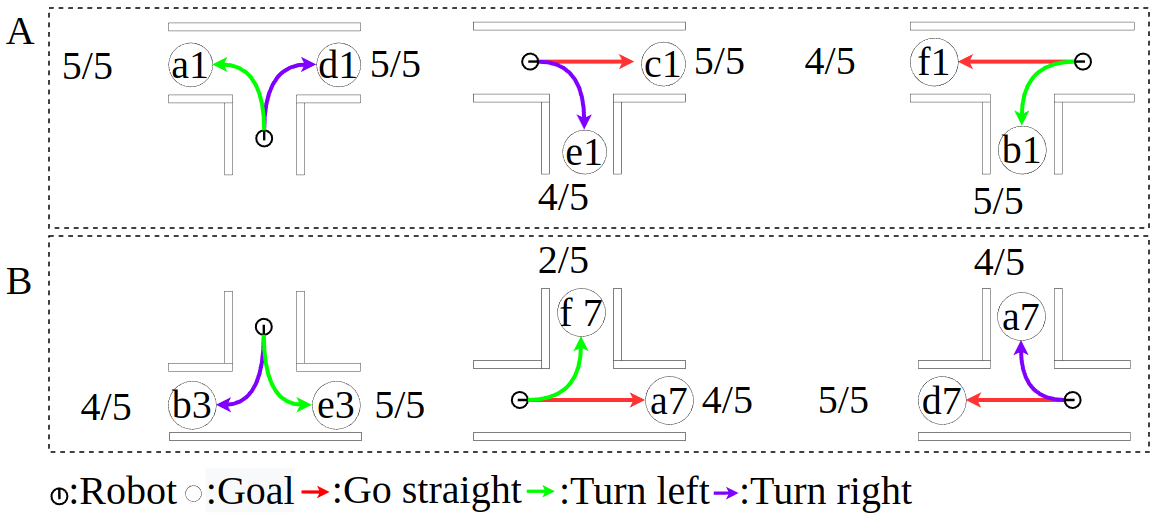
\includegraphics[keepaspectratio, scale=0.55]
        {images/10000step_act1.5.png}
   \caption{Experimental results for each moving pattern at 10000step by Approach 1+2}
   \label{Fig:10000step_act1.5}
  \end{figure}  
  
  % \vspace{0.5cm}

  \begin{table}[hbtp]
    \caption{Experimental results at 10000step by Approach 1+2}
    \label{table:result4}
    \centering
    \begin{tabular}{|c|c|c|}
      \hline
      Experiments & Step & Total results\\
      \hline
      Conventional & 60000 & 113/120(94.2\%)\\
      \hline
      Conventional & 10000 & 87/120(72.5\%)\\
      \hline
      Approach1 & 10000 & 99/120(82.5\%)\\
      \hline
      \textbf{Approach1+2} & \textbf{10000} & \textbf{109/120(90.8\%)}\\
      \hline
    \end{tabular}
  \end{table}

  % \vspace{1cm}

  \tabref{table:result4}からアプローチ1の実験より, 成功率が改善していることがわかる. また, 60000stepの実験と成功率を比較した場合, 約3\%ほどの差がある. 
  % \tabref{table:factor}
  以下に\figref{Fig:10000step_act1.5}における成功率が低い場所と要因を示す.
  \begin{itemize}
    \item f7\\
    4.1.2で示した経路の最後であり, 学習フェーズが終了する直前の三叉路である. そのため, データセットにf7のデータが加えられてから十分な学習ができていない
    \item a7, b3, e1\\
    これらは, 全て右折する場所である. \figref{Fig:hist}より, 他のコマンドのデータと比較して右折コマンドのデータが少ないことがわかる. このことから, 右折コマンドのデータを十分に学習できていない
  \end{itemize} 

  この2つの点から, 学習量を増加すると成功率が改善する可能性がある. そのため, 10000stepから20000stepに学習量を増加した実験結果を後述する.

  \newpage

  % \begin{table}[hbtp]
  %   \caption{Experimental results}
  %   \label{table:factor}
  %   \centering
  %   \begin{tabular}{|c|c|}
  %     \hline
  %     Points with low success rates & Primary factor\\
  %     \hline
  %     f7 & It is the last of the paths shown in 4.1.2, and the learning phase is terminated after passing through f7. Therefore, the data set has not been fully trained since the data of f7 was added to the dataset\\
  %     \hline
  %     a7, b3, e1 & 10000\\
  %     \hline
  %   \end{tabular}
  % \end{table}

  学習フェーズにおける目標経路からの距離によるデータの割合を\figref{Fig:hist_act_training}に示す. \par
  この図から, 学習器から得られた角速度を1.5倍にした場合, データの割合が目標経路付近では減少し, 目標経路から離れた場所では増加している. よって, アプローチ2を試みた結果, 学習フェーズでは目標経路から離れる行動が増えた. すなわち, 積極的に蛇行している可能性が高い.

  % \vspace{1cm}

  \begin{figure}[hbtp]
    \centering
   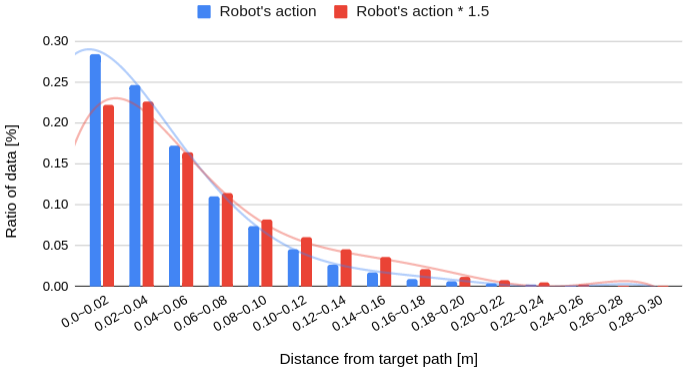
\includegraphics[keepaspectratio, scale=0.37]
        {images/hist_act_training.png}
   \caption{Ratio of data by distance from target path in learning phase}
   \label{Fig:hist_act_training}
  \end{figure}  

  % \newpage

  テストフェーズにおける目標経路からの距離によるデータの割合を\figref{Fig:hist_act_test}に示す. この図から, 学習器から得られた角速度を1.5倍にした場合, データの割合が目標経路付近では増加し, 目標経路から離れた場所では減少している. よって, アプローチ2を試みた結果, テストフェーズでは目標経路付近の行動が増えた. すなわち, アプローチ2を試みる前に比べ, より正確に経路追従行動を模倣している可能性が高い.

  \begin{figure}[hbtp]
    \centering
   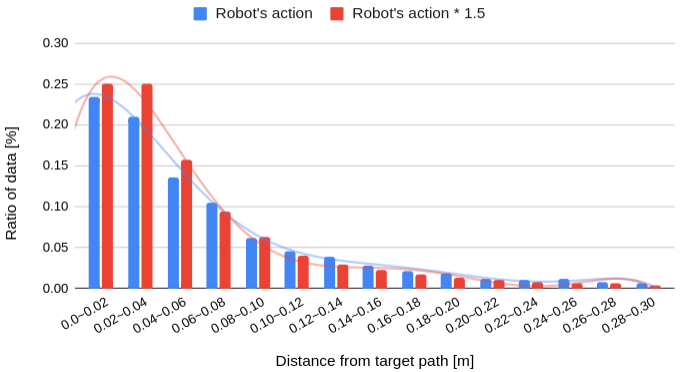
\includegraphics[keepaspectratio, scale=0.37]
        {images/hist_act_test.png}
   \caption{Ratio of data by distance from target path in test phase}
   \label{Fig:hist_act_test}
  \end{figure}  

  % \newpage

\end{itemize}

アプローチ1,2の実験を基に, 単に10000stepから20000stepに学習量を増やし, 実験した結果を下記に示す.

\figref{Fig:20000step_act1.5}は, それぞれの走行パターンにおいて正しく経路を選択し, 走行できた回数を表している. \tabref{table:result5} に実験ごとに全パターンの成功回数を合計した結果を示す. \tabref{table:result5} に示すように, 目標方向に従って 114/120 回, 正しい経路を選択する様子が見られた. また, 成功率が60000stepの実験と同程度になった. このことから, アプローチ1+2によって学習量が約67\%削減でき, 実験を実環境に移す際の問題が解決できたといえる. 

\begin{figure}[hbtp]
  \centering
 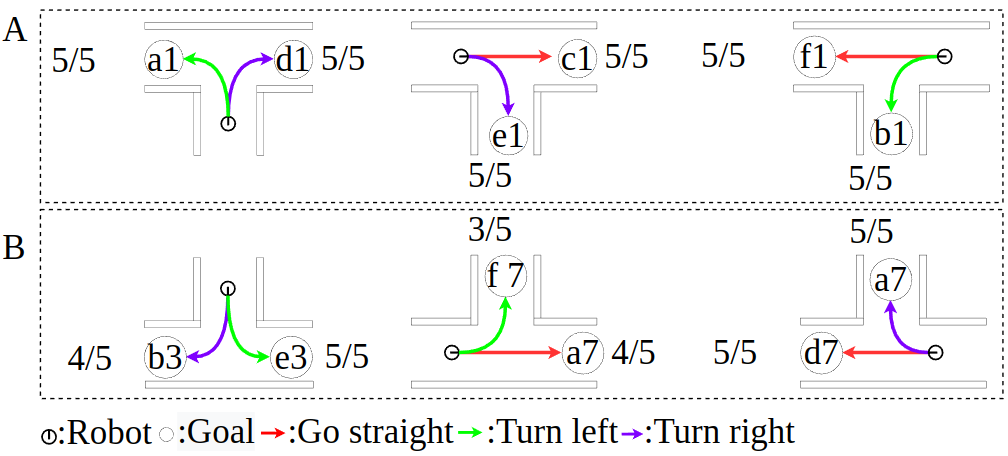
\includegraphics[keepaspectratio, scale=0.42]
      {images/20000step_act1.5.png}
 \caption{Experimental results for each moving pattern at 20000step by Approach 1+2}
 \label{Fig:20000step_act1.5}
\end{figure} 

\begin{table}[hbtp]
  \caption{Experimental results at 20000step by Approach 1+2}
  \label{table:result5}
  \centering
  \begin{tabular}{|c|c|c|}
    \hline
    Experiments & Step & Total results\\
    \hline
    Conventional & 60000 & 113/120(94.2\%)\\
    \hline
    Conventional & 10000 & 87/120(72.5\%)\\
    \hline
    Approach1 & 10000 & 99/120(82.5\%)\\
    \hline
    Approach1+2 & 10000 & 109/120(90.8\%)\\
    \hline
    \textbf{Approach1+2} & \textbf{20000} & \textbf{114/120(95\%)}\\
    \hline
  \end{tabular}
\end{table}

\newpage

%

%
%% Main Matter
\mainmatter{}
%
\chapter{序論}
\label{chap:introduction}
%
%\input{introduction/preface}
%
%!TEX root = ../thesis.tex

\section{背景}
近年, 機械学習を用いた自律走行に関する研究が盛んにされており, その中でカメラ画像を用いてロボットへ自律走行を行わせる研究もされている. Bojarskiら\cite{bojarski}は\figref{Fig:bojarski_train}に示すシステムで, 人間のドライバーが操作するステアリング角度と前方カメラ画像を用いて模倣学習を行った. また, \figref{Fig:bojarski_test}に示すように, 訓練したネットワークに画像を入力し, 生成される操舵指令を用いて走行を行う手法を提案した.

\vspace{0.5cm}

\begin{figure}[hbtp]
  \centering
 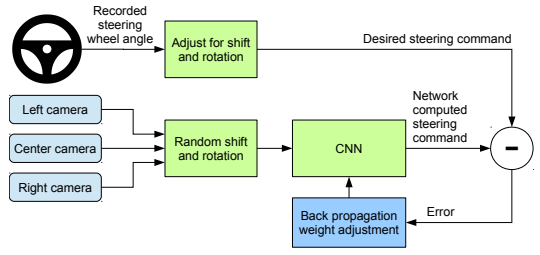
\includegraphics[keepaspectratio, scale=0.9]
      {images/bojarski_train.png}
 \caption{Training the neural network from \cite{bojarski}}
 \label{Fig:bojarski_train}
\end{figure}

\begin{figure}[hbtp]
     \centering
    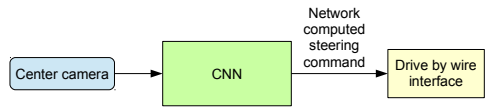
\includegraphics[keepaspectratio, scale=0.7]
         {images/bojarski_test.png}
    \caption{The trained network is used generate steering commands from a single front-facing center camera from \cite{bojarski}}
    \label{Fig:bojarski_test}
\end{figure}

\newpage

本研究室においても, 岡田ら\cite{okada1}\cite{okada2}は\figref{Fig:okada_structure}に示すようなシステムを用いて\figref{Fig:okada_nav}のように経路追従行動を模倣学習し, カメラ画像に基づいた経路追従行動を獲得した. このシステムでは, LiDAR, オドメトリを入力としたルールベース制御器(後述する”地図を用いたルールベース制御器”)による経路追従行動を前方カメラ画像を用いてend-to-endで模倣学習した. 

\vspace{2.5cm}

\begin{figure}[hbtp]
     \centering
     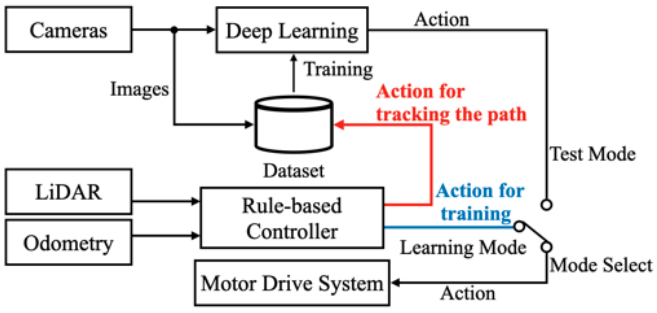
\includegraphics[keepaspectratio, scale=0.55]
          {images/okada_structure.png}
     \caption{Structure of the proposed system from \cite{okada1}}
     \label{Fig:okada_structure}
\end{figure}

\begin{figure}[hbtp]
     \centering
    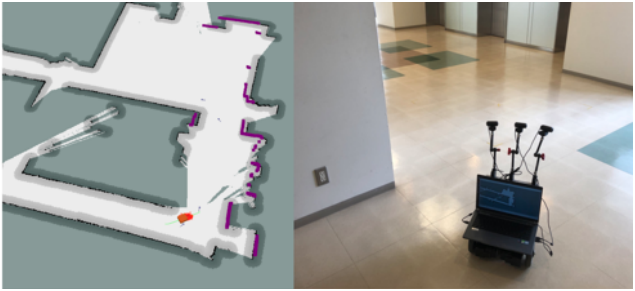
\includegraphics[keepaspectratio, scale=0.5]
         {images/okada_nav.png}
    \caption{A robot that follows a path using vision based on the proposed method from \cite{okada1}}
    \label{Fig:okada_nav}
\end{figure}

\newpage

上記の研究により, カメラ画像に基づいてロボットが学習した経路を周回可能であることが確認されている. 次に岡田らの研究(以下, 「従来手法」と称する)をベースに, \figref{Fig:road}のような分岐路において, 任意の経路を選択する機能の追加を検討する.

\vspace{1cm}

\begin{figure}[hbtp]
     \centering
    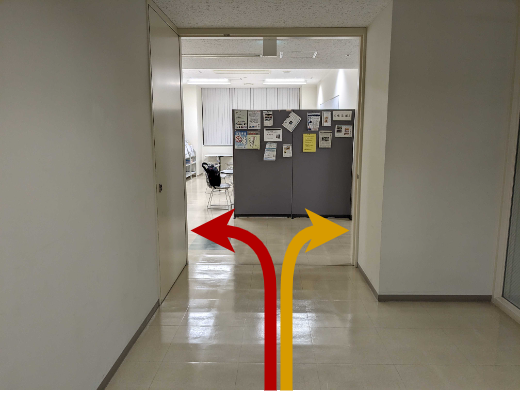
\includegraphics[keepaspectratio, scale=0.5]
         {images/road.png}
    \caption{A fork in the road where the direction of travel is not unique}
    \label{Fig:road}
\end{figure}

\newpage

本研究では, 従来手法をベースに「直進」, 「左折」, 「右折」の目標とする進行方向の情報(以下, 「目標方向」と称する)をデータセットと学習器へ与える. これにより, 訓練済みの学習器の出力を用いた走行において, 目標方向により任意の経路を選択可能とする機能の追加を提案する. 提案手法全体の流れを\figref{Fig:suggest_work}に示す. 

\begin{figure}[hbtp]
     \centering
    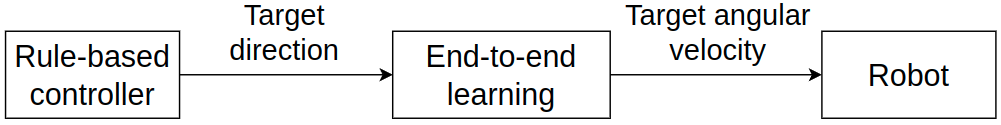
\includegraphics[keepaspectratio, scale=0.38]
         {images/suggest_work.png}
    \caption{Overall flow of the proposed method}
    \label{Fig:suggest_work}
\end{figure}

最終的にはカメラ画像を入力として, トポロジカルマップによって生成される目標方向に従って, 目的地まで移動する自律走行の手法を提案することを検討する. トポロジカルマップとは\figref{Fig:tsudanuma}に示すように, 重要な情報のみを残し, 分岐路などの目印(ノード)とつながり(エッジ)を持つ簡略化された地図である.

\vspace{0.5cm}

\begin{figure}[hbtp]
     \centering
    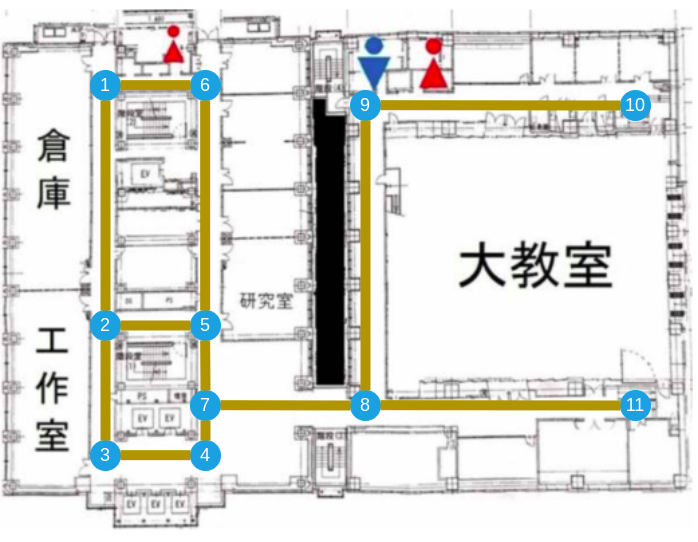
\includegraphics[keepaspectratio, scale=0.45]
         {images/tsudanuma.png}
    \caption{Topological map}
    \label{Fig:tsudanuma}
\end{figure}

カメラ画像とステアリング角度に, 条件を加えて学習を行う条件付き模倣学習によって, 自律移動を行う研究を述べる. Felipeら\cite{felipe}は前方カメラ画像, ステアリング角度, 加速度と「continue」, 「left」, 「straight」, 「right」からなるコマンドを入力とした\figref{Fig:felipe_network}のようなネットワークを用いて, \figref{Fig:felipe}に示すような実環境と都市環境のシミュレータ上で, 模倣学習のテスト時においてもコマンドによって制御可能であることを確認している.

\vspace{0.5cm}

\begin{figure}[hbtp]
     \centering
    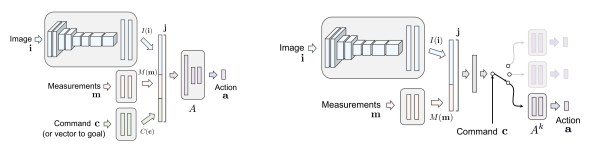
\includegraphics[keepaspectratio, scale=0.65]
         {images/felipe_network.png}
    \caption{Two network architectures for command-conditional imitation learning from \cite{felipe}}
    \label{Fig:felipe_network}
\end{figure}

\vspace{0.5cm}

\begin{figure}[hbtp]
     \centering
    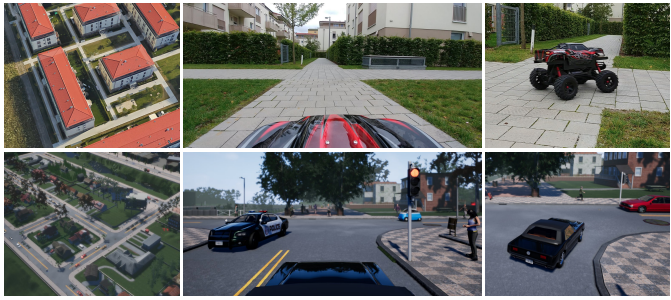
\includegraphics[keepaspectratio, scale=0.57]
         {images/felipe.png}
    \caption{End-to-end driving via conditional imitation learning from \cite{felipe}}
    \label{Fig:felipe}
\end{figure}

\newpage

また, Hawkeら\cite{hawke}は\figref{Fig:hawke}のような, 3つの前方カメラ画像と「go-straight」, 「turn-left」, 「turn-right」からなるコマンドを入力とする構造のモデルを用いて, 実環境での複雑な都市環境というシナリオで, 意思決定が可能なモデルをわずか30時間の学習データで学習可能であることを示している.

\vspace{3cm}

\begin{figure}[hbtp]
     \centering
    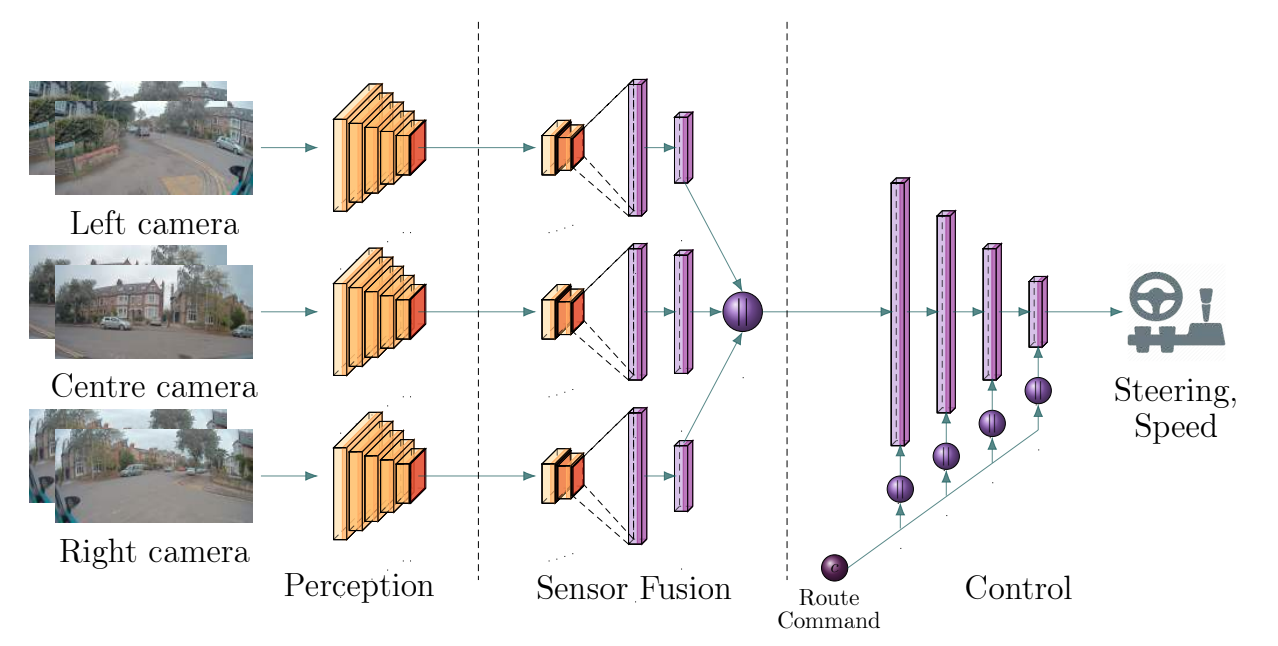
\includegraphics[keepaspectratio, scale=0.3]
         {images/hawke.png}
    \caption{Model structure from \cite{hawke}}
    \label{Fig:hawke}
\end{figure}

\newpage
%!TEX root = ../thesis.tex

\section{目的}
本研究では, 経路追従行動を模倣学習し, カメラ画像に基づいた経路追従行動を獲得する手法である岡田らの従来手法をベースとして, 分岐路において「直進」, 「左折」などのコマンドによる制御で任意の経路を選択可能にする機能の追加を提案する. また, シミュレータ上での実験を実環境に移す際に, 問題となった学習時間の長さについて, 2 つのアプローチの提案と検証を行った. さらに, 実環境における提案手法の有効性を検証することを目的とする.

% \begin{figure}[hbtp]
%   \centering
%  \includegraphics[keepaspectratio, scale=0.8]
%       {images/RaspberryPiMouse.png}
%  \caption{Example}
%  \label{Fig:Example}
% \end{figure}

% \newpage

%!TEX root = ../thesis.tex

\section{論文構成}
1章では, 本研究における背景,  及び目的を述べた. 2章では, 本研究で用いた深層学習の他所技術とベースとする従来手法について述べる. 3章では, 従来手法をベースにした, 提案手法を述べる. 4章では, シミュレータと実環境での実験を行う. 5章では, 本研究の結論を述べる.

% \begin{figure}[hbtp]
%   \centering
%  \includegraphics[keepaspectratio, scale=0.8]
%       {images/RaspberryPiMouse.png}
%  \caption{Example}
%  \label{Fig:Example}
% \end{figure}

\newpage

%

\chapter{要素技術}
\label{chap:technology}
%
本章では, 本研究で用いた深層学習に関連した要素技術と, ベースとなる従来手法にていて述べる.
%\input{introduction/preface}
%
%!TEX root = ../thesis.tex

\section{Deep learning}
Deep learningは, 画像や音声などのデータに特に適しており, 近年では自然言語処理や医療画像解析などさまざまな分野で活用されている.人間の脳のような深い層の構造を持つ人工ニューラルネットワークに基づく機械学習手法である. 人工ニューラルネットワークは, 入力データから出力データを予測するために, 多数のニューロンを用いて情報を処理する. この人工ニューラルネットワークを多層構造にすることで, より深い情報処理を行うことができる. これにより, 高度な識別や分類タスクなどを行うことを可能にしている. 一般的な構造を \figref{Fig:Neural network} に示す.

% \subsection{RoboCup}

\begin{figure}[hbtp]
  \centering
 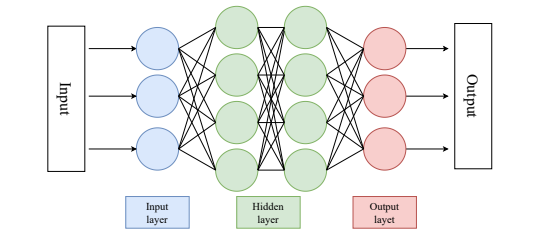
\includegraphics[keepaspectratio, scale=0.4]
      {images/deeplearning_model.png}
 \caption{Neural network}
 \label{Fig:Neural network}
\end{figure}

% \subsubsection{etc...}
\newpage

%!TEX root = ../thesis.tex

\section{end-to-end学習}
end-to-end学習とは, 人工ニューラルネットワークを使用して, 入力データから出力を直接
生成する方法のことを指す. \par 実世界における自動運転を例に挙げる. end-to-end学習を用いない場合, 人物や障害物などの物体認識, 車線の検出, 経路計画, ステアリングの制御など, 多くのタスクを解決する必要が
ある. しかし, end-to-endを用いることで, 先程のタスクを解決することなく, 車両が撮影したカメラ映像から直接, 運転操作を行うことができる. 
% \subsection{RoboCup}
\vspace{5cm}

\begin{figure}[hbtp]
  \centering
 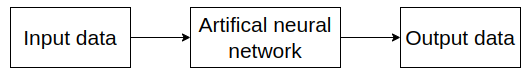
\includegraphics[keepaspectratio, scale=0.7]
      {images/end-to-end.png}
 \caption{Structure of end-to-end learning}
 \label{Fig:end-to-end}
\end{figure}

% \subsubsection{etc...}
\newpage

%!TEX root = ../thesis.tex

\section{Convolution Neural Network}
畳み込みニューラルネットワーク(convolutional neural network:CNN)は人工ニューラルネットワークのモデルの一種である. このモデルは, 画像や音声などの多次元の配列で表される複雑なデータを処理するために特別に設計されている. CNNは次のような特徴を持つ層で構成されている.
\begin{enumerate}
  \item 畳み込み層\\入力データをフィルタ(カーネル)を用いて特徴を抽出する.
  \item プーリング層\\特徴を残しつつ, 畳み込み層の出力を圧縮する. これにより, 画像であればピクセル数が減少し, 計算量が大幅に減らすことができる.
  \item 全結合層\\畳み込み層とプーリング層の出力をまとめて処理する.
\end{enumerate}

Krizhevskyら\cite{AlexNet}は\figref{Fig:AlexNet}で示すような, 8層のネットワークを用いて, 画像分類タスクをエラー率15.3\%で達成し, 画像分類コンペティションである ILSVRC(ImageNet Large Scale VisualRecognition Competition)2012で優勝した.
\begin{figure}[hbtp]
  \centering
 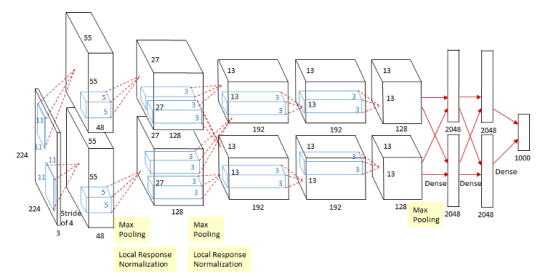
\includegraphics[keepaspectratio, scale=0.55]
      {images/AlexNet.png}
 \caption{AlexNet from \cite{AlexNet}}
 \label{Fig:AlexNet}
\end{figure}
\newpage
Simonyan\cite{simonyan}らはCNNの層の深さが精度に与える影響を調査した. 最大19層の深い畳み込みネットワークを評価した結果, モデルを深層にすることが分類精度に有利であることが示された.
ILSVRC2012の優勝モデルであるAlexNetは8層, ILSVRC2013で提案されたZFNetは同様の8層であることから, 当時のCNNとしては圧倒的に深い層を持つモデルであった. このような深い畳み込みネットワークは, 深層学習における重要な発展の一つとされている.
\begin{figure}[hbtp]
  \centering
 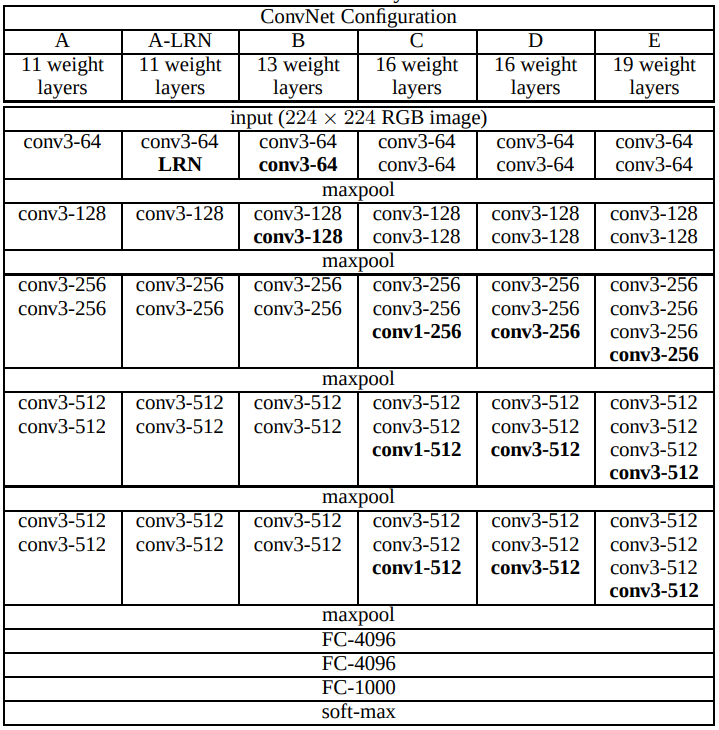
\includegraphics[keepaspectratio, scale=0.5]
      {images/VGG.png}
 \caption{VGG from \cite{AlexNet}}
 \label{Fig:VGG}
\end{figure}


% \vspace{5cm}

% \begin{figure}[hbtp]
%   \centering
%  \includegraphics[keepaspectratio, scale=0.7]
%       {images/end-to-end.png}
%  \caption{Structure of end-to-end learning}
%  \label{Fig:end-to-end}
% \end{figure}

% \subsubsection{etc...}
\newpage

%!TEX root = ../thesis.tex

\section{地図を用いたルールベースの制御器}
従来手法と提案手法において, 教師信号として用いる地図ベースの制御器について述べる. 地図ベースの制御器は, ROS Navigation\_stack\cite{navigation:online}へ移動目標の経由地点(waypoint)の指示を行うwaypoint\_nav\cite{waypoint_nav:online}を組み合わせたものである. ROS Navigation\_stackでは以下のような処理が行われる. 

\begin{itemize}
  \item ロボットの現在位置を推定する
  % \item 移動目標地点を決定する
  \item 移動目標地点までの経路を決定する
  \item 経路にしたがった行動をロボットに指示する
\end{itemize}

また, \figref{Fig:end-to-end}に示すように, 事前に生成した占有格子地図と測域センサ, オドメトリを用いて, 地図上での自己位置推定をParticle\_Filterによって確率的に行う「amcl」. 障害物認識などによる局所的, または地図全体の大域的なコスト計算, その結果に基づいた経路計画, それに従ったモータ指令を行う「move\_base」などのパッケージを統合した自律走行用のメタパッケージである. 従来手法, 提案手法ともにモータ指令を並進速度と角速度にわけた. 並進速度は一定とした.

% \vspace{5cm}

\begin{figure}[hbtp]
  \centering
 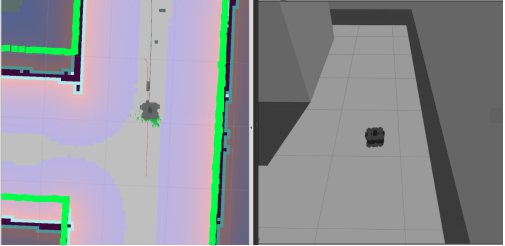
\includegraphics[keepaspectratio, scale=0.7]
      {images/navigation.png}
 \caption{A rule-based controller using a map}
 \label{Fig:navigation}
\end{figure}

% \subsubsection{etc...}
\newpage
%!TEX root = ../thesis.tex

\section{従来手法}
本研究のベースとなる岡田らの研究について述べる. 先に述べたように, 本論文では岡田らの手法を「従来手法」と呼ぶ. 従来手法は, 地図を用いたルールベース制御器が生成した走行を模倣学習し, 似た行動を画像を用いて行う手法である.\par
\figref{Fig:imitation_sys}に, 経路追従行動を視覚に基づいてオンラインで模倣するシステムを示す. 手法は模倣学習により, 学習器の訓練をする学習フェーズと訓練した結果を検証するテストフェーズにわかれる. なお, 両フェーズで用いる並進速度は一定の値を用いる.

\vspace{3cm}

\begin{figure}[hbtp]
  \centering
 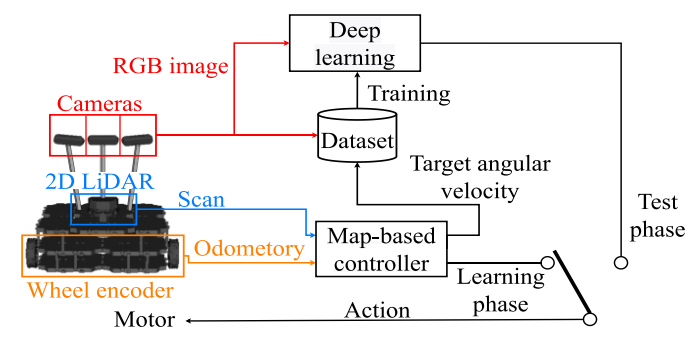
\includegraphics[keepaspectratio, scale=0.5]
      {images/imitation_sys.png}
 \caption{}
 \label{Fig:imitation_sys}
\end{figure}

\newpage

\subsection{学習フェーズ}
学習フェーズは, 模倣学習によって学習器の訓練を行うフェーズである. 地図を用いたルールベース制御器に, 測域センサとオドメトリのセンサ入力で自律走行を行う. 具体的には, ROS navigation\_stackパッケージを利用して, ロボットに自律移動させる. 学習フェーズでは, ロボットの中央, 左, 右に傾けて取り付けた3つのカメラを用いて画像を取得する. 自律移動させる際に, 取得するデータ量を増加させること及び, 過学習の抑制を目的として, \tabref{table:angular}に示すような処理を行う. また, 地図を用いたルールベース制御器の出力をそのまま模倣学習するのではなく, 少し蛇行するように自律移動させることで, 経路に戻るような挙動も学習できるようになっている. \figref{Fig:dakou}に示すように, 実際にロボットを制御する行動と経路に沿う行動を別に扱うことで, 常に経路に沿う行動をデータセットに加えることを可能にしている. ロボットに搭載したカメラ画像と地図を用いたルールベース制御器が出力するロボットのヨー方向の角速度の値をデータセットに加える. このデータセットを用いて, リアルタイムに模倣学習を行う. 岡田らの手法では, データセットの収集方法にいくつかのバリエーションがあるが, 本論文では前報\cite{okada2}において最も経路追従の成功率が高い手法を用いて, ロボットに模倣学習をさせる.

\begin{table}[hbtp]
  \caption{Angular velocity offset}
  \label{table:angular}
  \centering
  \begin{tabular}{|c|c|}
    \hline
    Left camera  & Angular velocity of a rule-based controller using a map + 0.2 rad/s\\
    \hline
    Center camera  & Angular velocity of a rule-based controller using a map  \\
    \hline
    Right camera  & Angular velocity of a rule-based controller using a map - 0.2 rad/s   \\
    \hline
  \end{tabular}
\end{table}

\begin{figure}[hbtp]
  \centering
 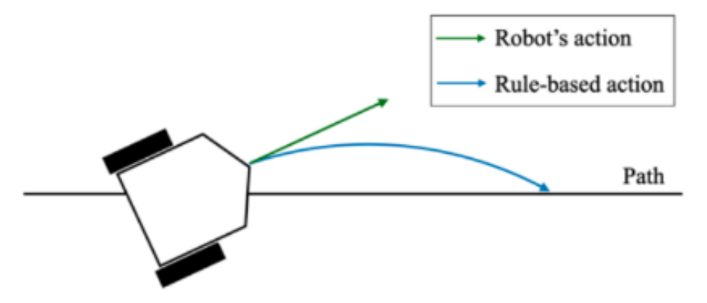
\includegraphics[keepaspectratio, scale=0.4]
      {images/dakou.png}
 \caption{Output of rule-based controller using a map and actual robot behavior}
 \label{Fig:dakou}
\end{figure}

\subsection{テストフェーズ}
学習器の訓練後, テストフェーズへ移行する. このフェーズでは, 学習器にカメラ画像を入力し, 出力されるヨー方向の角速度を用いて自律移動することで, 訓練後の学習結果を評価する. 

% \vspace{3cm}

% \subsubsection{etc...}
\newpage
%

\chapter{提案手法}
\label{chap:suggest}
%
本章では, 従来手法をベースとする提案手法についての概要, 提案手法における学習フェーズ, テストフェーズ, 目標方向, ネットワーク構造についての5節に分けて述べる.
%\input{introduction/preface}
%
%!TEX root = ../thesis.tex

\section{提案手法の概要}
本研究では, 従来手法をベースに「直進」, 「左折」, 「右折」の目標とする進行方向の情報(以下, 「目標方向」と称する)をデータセットと学習器へ追加する. これにより, 訓練済みの学習器の出力を用いた走行において, 目標方向により任意の経路を選択可能とする機能の追加を行った. なお, 追加した要素以外は従来手法と同様である. 提案手法全体の流れを\figref{Fig:suggest_work}に示す. 

\begin{figure}[hbtp]
     \centering
    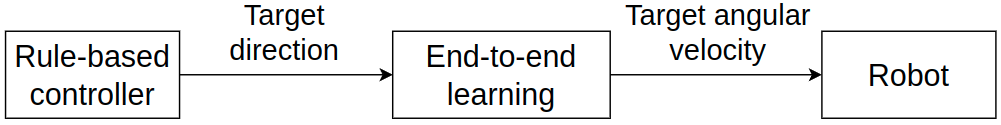
\includegraphics[keepaspectratio, scale=0.38]
         {images/suggest_work.png}
    \caption{Overall flow of the proposed method}
    \label{Fig:suggest_work}
\end{figure}

最終的にはカメラ画像を入力として, トポロジカルマップによって生成される目標方向に従って, 目的地まで移動する自律走行の手法を提案することを検討する. トポロジカルマップとは\figref{Fig:tsudanuma}に示すように, 分岐路などの目印(ノード)とつながり(エッジ)を持つ簡略化された地図である.

% \vspace{0.5cm}
\newpage

\vspace{0.5cm}

\begin{figure}[hbtp]
     \centering
    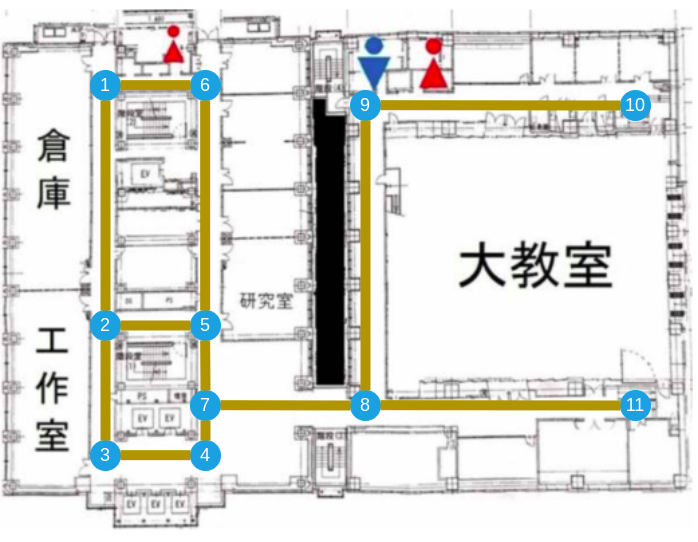
\includegraphics[keepaspectratio, scale=0.45]
         {images/tsudanuma.png}
    \caption{Topological map}
    \label{Fig:tsudanuma}
\end{figure}

% 従来手法で用いていたデータセットと学習器の入力へ, 「直進」「左折」などの目標方向を追加する. これにより, 学習器の出力による自律移動において, 経路を選択する機能の追加を行った. なお, 追加した要素以外は従来手法と同様である.

% \subsection{RoboCup}

% \begin{figure}[hbtp]
%   \centering
%  \includegraphics[keepaspectratio, scale=0.4]
%       {images/deeplearning_model.png}
%  \caption{Neural network}
%  \label{Fig:Neural network}
% \end{figure}

% \subsubsection{etc...}

\newpage

%!TEX root = ../thesis.tex

\section{学習フェーズ}
提案手法で用いる学習フェーズを\figref{Fig:suggest_learning_sys}に示す. 経路追従行動を行う地図ベースの制御器から目標方向を生成し, データセットに加えている. 提案手法では, \figref{Fig:overview}に示すようにLiDARとオドメトリを入力とする地図ベースの制御器による経路追従行動を, カメラ画像と目標方向を用いて模倣学習する.

\begin{figure}[hbtp]
  \centering
 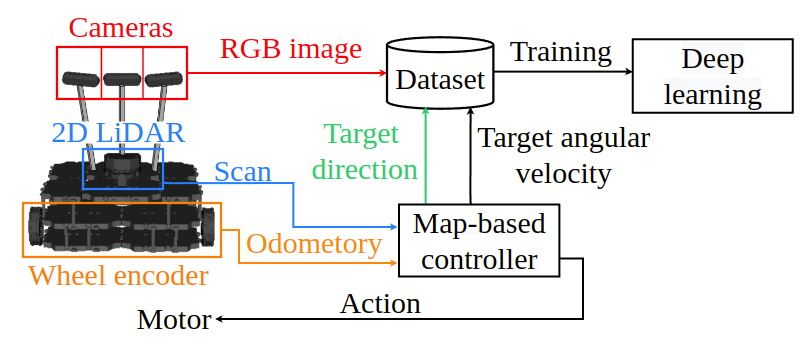
\includegraphics[keepaspectratio, scale=0.45]
      {images/suggest_learning_sys.png}
 \caption{Learning phase system of proposed method}
 \label{Fig:suggest_learning_sys}
\end{figure}

\begin{figure}[hbtp]
  \centering
 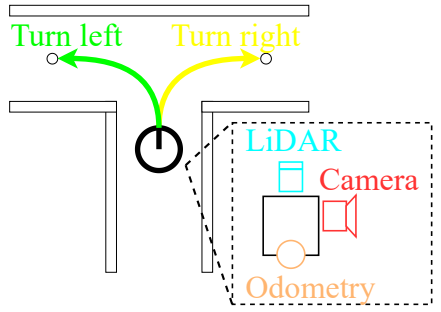
\includegraphics[keepaspectratio, scale=0.6]
      {images/overview.png}
 \caption{Overview learning phase}
 \label{Fig:overview}
\end{figure}

% \subsubsection{etc...}
\newpage

%!TEX root = ../thesis.tex

\section{テストフェーズ}
提案手法におけるテストフェーズでは\figref{Fig:suggest_test_phase}で示すように, 従来手法のシステムから新たに目標方向を学習器の入力へ追加した. なお, テストフェーズも学習フェーズと同様に, 地図を用いたルールベース制御器から目標方向を生成している. 
\par
最終的には, 目的地までカメラ画像のみで自律移動させることを目標としているため, 目標方向を画像から自動的に作成する仕組みが必要となるが, それは今後の課題として, 本論文では議論しない.
% そのため, 以下のようなROSパッケージを作成している\cite{weighted_graph}.

% \begin{itemize}
%      \item GUI上で目的地(ノード)を設定すると, ダイクストラ法でノード間の距離を考慮した経路探索を行う. その後, 経由するノードの位置関係から目標方向を自動生成し, 同時にカメラ画像からノードの場所検出を行い, 適切な目標方向に切り替える.
% \end{itemize}

% figに動作の様子を示す. 
\par
学習フェーズで訓練した学習器の出力により自律走行しながら, 目標方向によって任意の経路を選択する.

\vspace{1cm}

\begin{figure}[hbtp]
  \centering
 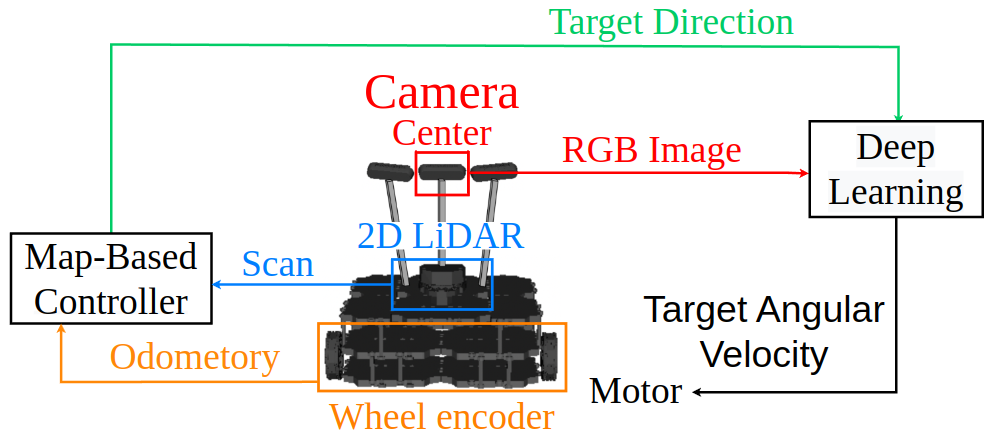
\includegraphics[keepaspectratio, scale=0.38]
      {images/test_propose.png}
 \caption{Test phase system of proposed method}
 \label{Fig:suggest_test_phase}
\end{figure}

% \subsubsection{etc...}
\newpage

%!TEX root = ../thesis.tex

\section{目標方向}
本研究で用いた目標方向と, そのデータ形式である目標方向指令について述べる. 目標方向を\figref{Fig:direction}に示す. 目標方向を経路と分岐路において「道なり」に走行(Go straight), 分岐路において「直進(Go straight)」, 「左折(Turn left)」, 「右折(Turn right)」の3つとする. なお, \cite{mech}では「道なり(continue)」, 「直進(Go straight)」, 「左折(Turn left)」, 「右折(Turn right)」からなる4つのコマンドを用いていたが, 「道なり」と「直進」のコマンドに対応する行動がほぼ同一であったため, 本研究ではコマンドを1つ減らし, 3コマンドとしている.

\begin{figure}[hbtp]
  \centering
 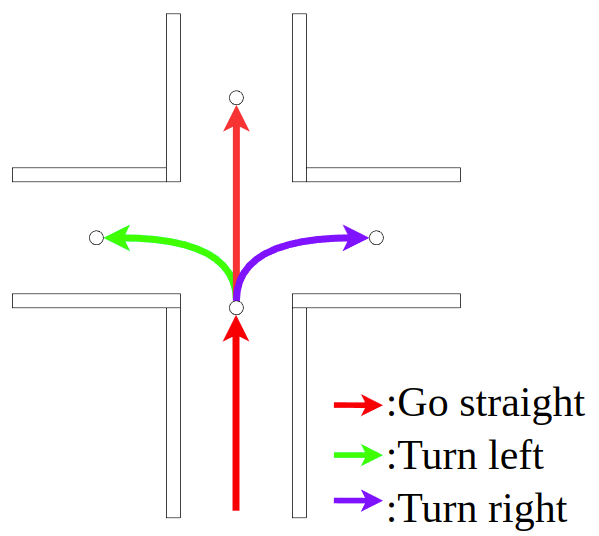
\includegraphics[keepaspectratio, scale=0.38]
      {images/direction.png}
 \caption{Target direction}
 \label{Fig:direction}
\end{figure}

学習器には, 上記の3つの目標方向を要素数3, 次元数1のint型の配列で表現した”目標方向指令”を入力する. 目標方向指令のデータ形式を\tabref{table:direction}に示す.

\begin{table}[hbtp]
  \caption{Target direction list}
  \label{table:direction}
  \centering
  \begin{tabular}{|c|c|c|c|}
    \hline
    Target Direction  & Go straight & Turn left & Trun right\\
    \hline
    Data & [100, 0, 0] & [0, 100, 0] & [0, 0, 100]\\
    \hline
  \end{tabular}
\end{table}

% \begin{figure}[hbtp]
%   \centering
%  \includegraphics[keepaspectratio, scale=0.45]
%       {images/direction.png}
%  \caption{Learning phase system of proposed method}
%  \label{Fig:direction}
% \end{figure}

% \subsubsection{etc...}
\newpage

%!TEX root = ../thesis.tex

\section{ネットワーク構造}
提案手法で用いた学習器のネットワークを\figref{Fig:network_structure}に示す. また, ハイパーパラメータについてtableに示す. 64x48のRGB画像を入力とする入力層1層, 畳み込み層3層, 全結合層2層を持つ6層のCNNと, このCNNの出力と目標方向指令を入力する入力層1層, 全結合層2層, 出力層1層の全10層から構成されている. 出力はヨー方向の角速度である.

\begin{figure}[hbtp]
  \centering
 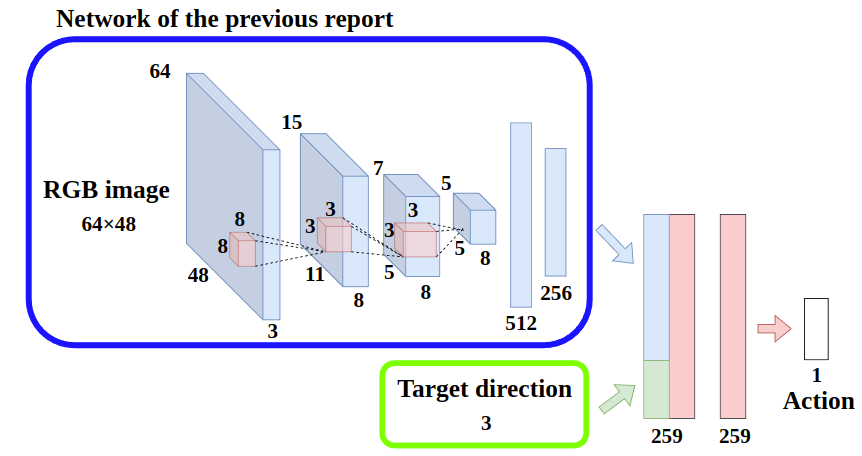
\includegraphics[keepaspectratio, scale=0.43]
      {images/network_structure2.png}
 \caption{Method network}
 \label{Fig:network_structure}
\end{figure}

\begin{table}[hbtp]
  \caption{Parameters of network}
  \label{table:param1}
  \centering
  \begin{tabular}{|c|c|}
    \hline
    Input data & Image(64x48 pixels, RGB channels), Target direction \\
    \hline
    Optimizer & Adam($alpha = 0.001, beta1 = 0.9, beta2 =  0.999, eps = 1e^{-2}$)\\
    \hline
    Loss function & Softmax-cross-entropy\\
    \hline
    Output data & Angular velocity\\
    \hline
  \end{tabular}
\end{table}

% \begin{figure}[hbtp]
%   \centering
%  \includegraphics[keepaspectratio, scale=0.45]
%       {images/network_structure.png}
%  \caption{Learning phase system of proposed method}
%  \label{Fig:network_structure}
% \end{figure}

% \subsubsection{etc...}
\newpage

%

%ここにディレクトリのパスを追加していく
%
%% Back Matter
\backmatter{}
%
%!TEX root = ../thesis.tex
%\bibliographystyle{plain}
\bibliographystyle{junsrt}
%\bibliography{report}
\nocite{*}
\bibliography{main_bibliography}
%
%!TEX root = ../thesis.tex
\chapter*{付録}
\addcontentsline{toc}{chapter}{付録}

\leftline{\textbf{動画}}

実験の結果から得られたモデルを用いて, 中間層の可視化を行った状態で学習器の出力において走行させた際の動画を記録した. CNNが通路の特徴(輪郭, または壁と床の境界線)を捉えるように学習を行ったことが見て取れる. 以下にアップロードした動画のURLを掲載する.\\
\url{https://youtu.be/JusGVH6ejFg}
%
%!TEX root = ../thesis.tex
\chapter*{謝辞}
\addcontentsline{toc}{chapter}{謝辞}

本研究を進めるにあたり,1年に渡り, 熱心にご指導を頂いた林原靖男教授に深く感謝いたします.ロボット設計制御研究室の皆様には, ご意見, ご協力頂き感謝申し上げます. 特に, 春山健太氏には, 研究の着想や実験など多くの助言をして頂きましたことを心より感謝いたします.
%



%

\end{document}
